\documentclass[a4paper, 11pt,reqno]{article}
\input{/Users/olivierglorieux/Desktop/BCPST/2020:2021/preambule.tex}


\newif\ifshow
\showtrue
\input{/Users/olivierglorieux/Desktop/BCPST/2021:2022/ifshow.tex}


\geometry{hmargin=2.0cm, vmargin=2cm}

\author{Olivier Glorieux}
\begin{document}
\title{DM 16}


\vspace{1cm}
\begin{exercice}[d'après Agro 2016]
Soient $u$ et $v$ deux vecteurs de $\mathbb{R}^{n}$.
Le produit scalaire de $u$ et $v$ est notée $u \cdot v$, on note $u^{2}=u \cdot u$ et l'on a $u^{2}=\|u\|^{2}$.


Si $E$ désigne un sous-espace vectoriel de $\mathbb{R}^{n}$, on note 

$$E^{\perp} =\{ x \in \R^n \, |\,  \forall y\in E, \langle x,y\rangle=0\}.$$
$E^{\perp}$ s'appelle le sous-espace orthogonal à $E$, il est formé de tous les vecteurs qui sont orthogonaux à $E$. 

0. Soit $E$ un sous-espace vectoriel de $\R^n$. Montrer que $E^{\perp}$ est un sous-espace vectoriel de $\R^n$. \\

Dans $\mathbb{R}^{3}$ on considère les vecteurs $u=(1,2,3)$ et $v=(-3,1,5)$.
\begin{enumerate}
\item Déterminer la dimension du sous-espace vectoriel $E$ de $\mathbb{R}^{3}$ engendré par la famille $(u, v)$.
\item  Déterminer le nombre réel $\lambda$ tel que le vecteur $v^{\prime}=u+\lambda v$ soit orthogonal à $u$.

\item Pour tout vecteur $w$ de $\mathbb{R}^{3}$, on définit le vecteur $w^{\prime}$ par $w^{\prime}=w-\frac{(w \cdot u)}{\|u\|^{2}} u-\frac{\left(w \cdot v^{\prime}\right)}{\left\|v^{\prime}\right\|^{2}} v^{\prime}$.
\begin{enumerate}
\item  Montrer que pour tout vecteur $w$, on a $w^{\prime} \in E^{\perp}$.
Dans la suite, on suppose que $w=(-2,3,2)$.
\item  Montrer que $w \notin E$ et $w \notin E^{\perp}$.
\item  Déterminer le vecteur $w^{\prime}$ associé à $w$.
\item  Montrer que la famille $\left(u, v^{\prime}, w^{\prime}\right)$ est une base de $\R^3$.
\end{enumerate}

\end{enumerate}

\end{exercice}

\begin{correction}
\begin{enumerate}
\item Les deux vecteurs $u$ et $v$ ne sont pas proportionnels, la famille $(u,v)$  est donc une famille libre. 
Ainsi $(u,v)$ est une base de $Vect(u,v)$
\conclusion{ $Vect(u,v)$ est donc de dimension 2.}
\item On chercher $\lambda \in \R$ tel que 
$$\langle u+\lambda v , u \rangle =0 \quad (E)$$ 
Le vecteur $u+\lambda v$ a pour coordonnées : $(1-3\lambda, 2+\lambda , 3+5 \lambda)$ donc 
$$(E)\equivaut (1-3\lambda)\times 1 + (2+\lambda) \times 2 + (3+5 \lambda ) 3 =0$$
Ce qui donne 
$$(-3+2+15)\lambda +(1+4+9)=0$$
D'où \conclusion {$ \lambda =-1$}


\item \begin{enumerate}
\item Montrons que $w'$ comme défini dans l'énoncé appartient à $E^\perp$ c'est à dire que pour tout vecteur $y$ de $E$, $\langle w', y \rangle =0$. 
Calculons tout d'abord 
$\langle w', u \rangle$ et $\langle w', v' \rangle$.

On a 
\begin{align*}
\langle w', u \rangle &=  \langle w-\frac{(w \cdot u)}{\|u\|^{2}} u-\frac{\left(w \cdot v^{\prime}\right)}{\left\|v^{\prime}\right\|^{2}} v^{\prime} , u \rangle\\
&= \langle w , u \rangle - \frac{(w \cdot u)}{\|u\|^{2}} \langle u , u \rangle - \frac{\left(w \cdot v^{\prime}\right)}{\left\|v^{\prime}\right\|^{2}}\langle v^{\prime} , u \rangle
\end{align*}
par linéarité du produit scalaire


Or $\langle v^{\prime} , u \rangle= 0$ d'après la définition de $\lambda $ dans la question précédente et $ \langle u , u \rangle =\|u\|^2$ par définition de la norme. 

Donc 

\begin{align*}
\langle w', u \rangle &= \langle w , u \rangle - \langle w \cdot u \rangle \\
&=0
\end{align*}

De manière identique on trouve 
On a 
\begin{align*}
\langle w', v' \rangle &=  \langle w-\frac{(w \cdot u)}{\|u\|^{2}} u-\frac{\left(w \cdot v^{\prime}\right)}{\left\|v^{\prime}\right\|^{2}} v^{\prime} , v' \rangle\\
&= \langle w , v' \rangle - \frac{(w \cdot u)}{\|u\|^{2}} \langle u , v' \rangle - \frac{\left(w \cdot v^{\prime}\right)}{\left\|v^{\prime}\right\|^{2}}\langle v^{\prime} , u' \rangle
\end{align*}
par linéarité du produit scalaire


Or $\langle  u , v^{\prime} \rangle= 0$ d'après la définition de $\lambda $ dans la question précédente et $ \langle v' , v' \rangle =\|v'\|^2$ par définition de la norme. 



Donc 

\begin{align*}
\langle w', v' \rangle &= \langle w , v' \rangle - \langle w \cdot v' \rangle \\
&=0
\end{align*}

Ainsi $w'$ est orthogonal à $u$ et $v'$. De plus $v'$  est une combinaison linéaire de $u$ et $v$ et $(u,v)$ est une base de $E$ donc, $(u,v')$ est est aussi une base de $E$. Ainsi pour tout $x\in E$ il existe $a, b\in /R^2$ tel que $x= au +bv'$ et donc :
\begin{align*}
\langle w'  , x \rangle &= \langle w', au +bv\rangle\\
									 &= a\langle w', u\rangle b \langle w' , v\rangle\\
									 &= 0
\end{align*}
d'après les calculs effectués précédemment. 

\conclusion{ Pour tout $x\in E$ , $\langle w'  , x \rangle=0$, donc $w' \in E^\perp$}

\item Supposons par l'absurde que $w\in E$, dans ce cas il existe $a, b\in \R^2$ tel qu e
$au +bv =w$. Les réels  $(a,b)$ sont donc solutions du systèmes:
$$\left\{ \begin{array}{cc}
a -3b &=-2\\
2a+b &= 3\\
3a +5b&= 2
\end{array}\right.$$
On échelonne en faisant $L_2\leftarrow L_2 -2L_1$ et $L_3\leftarrow L_3 -3L_1$. 
$$\left\{ \begin{array}{ccc}
a &-3b &=-2\\
&7b &= 7\\
&14b&= 8
\end{array}\right. \equivaut 
\left\{ \begin{array}{ccc}
a &-3b &=-2\\
&b &= 1\\
&0&= -6
\end{array}\right. 
$$

\conclusion{ Le système n'admet pas de solution, donc $w\notin E$. }


Montrons désormais que $w\notin E^\perp$. On a 
 $$\langle w , u \rangle = -2 +6 +6=10\neq 0$$ 
 Donc $w$ n'est pas orthogonal à $u\in E$ donc 
 \conclusion{ $w\notin E^\perp$}


\item D'après la question 2 on a $v'= (4,1,-2)$. Calculons maintenant tous les termes dans la définition de $w'$. 
\begin{align*}
\langle w , u \rangle&= 10\\
\|u\|^2 &= 1+4+9=14\\
\langle w , v' \rangle&= -8+3-4=-9\\
\|v'\|^2 &= 16+1+4=21
\end{align*}

Donc 
\begin{align*}
w' & =w - \frac{10}{14} u - \frac{-9}{21}v'\\
	&= (-2,3,2) - \frac{5}{7} (1,2,3) +\frac{3}{7} (4,1,-2)\\
	&= \frac{1}{7} (-14-5+12, 21-10 +3, 14-15-6)\\
	&=\frac{1}{7} (-7, 14, -7)\\
	&= (-1,2,-1)
\end{align*}

\conclusion{ $w' =(-1,2,1)$}
\item 
Soit $a,b,c\in \R^3$ tel que $au+bv'+cw'=0$  (de quel 0 parle-t-on ici ? )
En prenant le produit scalaire avec $u$ on obtient 
$$\langle au+bv'+cw', u \rangle = 0$$
 (et de quel 0 parle-t-on là ? )
 
 Donc par linéarité du produit scalaire : 
 $$a \langle u, u \rangle+b\langle v', u \rangle+c\langle w', u \rangle=0$$
Or $\langle v', u \rangle= \langle w', u \rangle=0$
Donc  $$a \|u\|^2=0$$
Comme $u$ n'est pas le vecteur nul, $\|u\|^2 \neq 0$ donc $a=0$ 

On a donc $bv'+cw'=0$  (de quel 0 parle-t-on ici ? )
En prenant le produit scalaire avec $v'$ on obtient 
$$\langle bv'+cw', v' \rangle = 0$$
 (et de quel 0 parle-t-on là ? )
 
 Donc par linéarité du produit scalaire : 
 $$b\langle v', v'\rangle+c\langle w', v' \rangle=0$$
Or $\langle w', v' \rangle=0$
Donc  $$b\|v'\|^2=0$$
Comme $v'$ n'est pas le vecteur nul, $\|v'\|^2 \neq 0$ donc $b=0$ 

On a donc $cw'=0$
Comme $v'$ n'est pas le vecteur nul, $c=0$ 

Ainsi la famille ($u,v',w') $ est libre. De plus comme elle est de cardinal 3 dans un espace de dimension 3 ($\R^3$)  on conclut que 
\conclusion{ $(u,v',w') $ est une base de $\R^3$ }











\end{enumerate}


\end{enumerate}
\end{correction}



\begin{probleme}
Le but de ce problème est d'étudier la fonction définie par : 
$$g : x \mapsto \int_x^{x^2} \frac{dt}{\ln(t)}.$$
\begin{enumerate}
\item Etude globale : 
\begin{enumerate}
\item Justifier que $g$ est bien définie sur $\cD_g = ]0,1[\cup ]1,+\infty[$. 
\item Montrer que $g$ est positive sur $\cD_g$. 
\item Soit $F$ une primitive (qu'on ne cherchera pas à calculer) de $t\mapsto \frac{1}{\ln(t)}$ sur $]0,1[$. Exprimer $g$ à l'aide de $F$ pour tout $x\in ]0,1[$.
\item En déduire  que $g$ est dérivable sur $\cD_g$  et montrer que pour tout $x\in ]0,1[$ : 
$$g'(x) =\frac{x-1}{\ln(x)}$$
(C'est LA question à faire)
\item Par un raisonnement identique montrer que $g$ est dérivable sur $D_g$. 
\item Montrer que $g$ est de classe $\cC^\infty$ sur $\cD_g$. 
\item Etudier les variations de $g$ sur $\cD_g$. (les limites aux bornes ne sont pas demandées pour cette question) 
\end{enumerate}
\item Etude au voisinage de $0$
\begin{enumerate}
\item Montrer que :
$$\forall x\in ]0,1[\quad \frac{x(x-1)}{2\ln(x)}\leq g(x)\leq \frac{x(x-1)}{\ln(x)}$$
On fera très attention aux signes dans les inégalités. 
\item En déduire que $g$ se prolonge par continuité en $0$ et préciser la valeur de ce prolongement. 
Par la suite, on note encore $g$ la fonction continue, prolongée en $0$
\item Montrer que $g$ est dérivable à droite en $0$ et préciser $g'(0)$. 
\end{enumerate}
\item Etude au voisinage de $1$.
\begin{enumerate}
\item Calculer la limite  $\lim_{t\tv 1} \frac{1}{\ln(t)} -\frac{1}{t-1}$
\item En déduire qu'il existe $\eta > 0 $ tel que pour tout $t\in [1-\eta, 1+\eta]\setminus \{ 1\} $:
$$ \left|\frac{1}{\ln(t)} -\frac{1}{t-1}\right|\leq 1$$
\item Conclure  que $g$  est prolongeable par continuité en $1$. 
\end{enumerate}


\end{enumerate}

\end{probleme}




\begin{correction}
\begin{enumerate}
\item Etude globale
\begin{enumerate}
\item On note $f$ la fonction définie par $f(x)=\frac{1}{\ln(x)}$.
Cette fonction est définie pour tout $x\in \R$ tel que $\ln(x)$ soit défini, c'est-à-dire $x>0$ et tel que $\ln(x)\neq0$, c'est-à-dire $x\neq 1$. On a donc $D_f =  ]0,1[\cup ]1,+\infty[$. 

La fonction $f$ est continue  sur son ensemble de définition comme quotient de fonction usuelle, elle admet donc une primitive sur $]0,1[$ et sur $]1,+\infty[$. \footnote{Il faut faire attention ici que \underline{l'intervalle} définie par les bornes de l'intégrale ne contiennent pas des points où $f$ n'est pas définie. } 

Notons $F_1$ une primitive sur $]0,1[$. Pour tout $x\in ]0,1[$, on a $x^2\in ]0,1[$ et ainsi $$g(x)=F_1(x^2)-F_1(x)$$ est bien définie sur $]0,1[$. 

De la même façon, en notant $F_2$ une primitive sur $]1,+\infty[$. Pour tout $x\in ]1,\infty[$, on a $x^2\in ]1,\infty[$ et ainsi $$g(x)=F_2(x^2)-F_2(x)$$ est bien définie sur $]1,\infty[$. 

Finalement 
\conclusion{ $D_g =]0,1[\cup ]1,+\infty[$}
\item 
Nous reprenons les notations de la question 1. Pour tout $x\in ]0,1[, $ $x^2<x$ ainsi $g(x) = -\int_{x^2}^x f(t)dt$, où les bornes d'intégration sont ordonnées dans le sens croissant. Maintenant pour $x\in ]0,1[$,  $[x^2,x] \subset ]0,1[$ or pour $t\in ]0,1[$, $f(t) < 0$. 
\conclusion{ Ainsi $g(x)>0$ sur $]0,1[$. }

Pour $x>1$, on a $x^2>x$ et les bornes sont déjà bien ordonées. De plus $\frac{1}{\ln(t)}>0$ pour tout $t>1$ et 
\conclusion{ On a bien $g(x)>0$ sur $]1,+\infty[$. }


\item Cf question 1 : $g(x) = F (x^2) - F(x)$
\item Nous reprenons les notations de la question 1. Par définition on  a
$g(x) = F_1 (x^2) - F_1(x)$ pour $0<x<1$ et $g(x) = F_2 (x^2) - F_2(x)$ pour $x>1$. Or par définition d'une primitive les fonctions $F_1, F_2$ sont dérivables sur leur ensemble de définition. Donc $g$ est dérivable en tant que composée et somme de fonctions dérivables. 

On  a pour tout $x<1$ : $g'(x) = 2xF_1'(x^2) - F_1'(x)$. Or $F_1'(x) =f(x)$ et donc 
$g'(x) =\frac{2x}{\ln(x^2)}-\frac{1}{\ln(x)},  $ en simplifiant et factorisant on obtient : 
\conclusion{$g'(x) = \frac{x-1}{\ln(x)}$}

\item Les calculs sont identiques sur $]1,+\infty[$. 

\item La fonction $g'$ est de classe $\cC^\infty$ sur $\cD_g$ comme quotient de fonction $\cC^\infty$. \conclusion{Ainisi $g$ est de classe $\cC^\infty$ sur $\cD_g$. }

\item On  a vu que pour tout $x\in \cD_g$ on a 
$$g'(x) = \frac{x-1}{\ln(x)}$$
On obtient le tableau de signe/variations suivant :

\begin{tikzpicture}
   \tkzTabInit{$x$ / 1 , $x-1$ / 1, $\ln(x)$ / 1, $g'(x)$/1, $g(x)$ /1.5 }{$0$, $1$, $+\infty$}
   \tkzTabLine{, -, z, +, }
      \tkzTabLine{, -, z, +, }
            \tkzTabLine{, +, d, +, }
           
\tkzTabVar{-/ , R/, +/ }
 \tkzTabIma{1}{3}{2}{  }
  % \tkzTabVal{1}{2}{0.5}{}{} 
\end{tikzpicture}





\end{enumerate}
\item Etude au voisinage de $0$. 
\begin{enumerate}
\item Soit $x\in ]0,1[$, alors comme on l'a vu précédemment 
$g(x)  = -\int_{x^2}^x f(t)dt$ où les bornes de l'intégrales sont bien ordonnées. 
Par ailleurs pour tout $t\in [x^2,x]$ on a $\ln(x^2)\leq \ln(t) \leq \ln(x)<0$ par croissance du logarithme. Et donc 
$$\frac{1}{\ln(x)}\leq \frac{1}{\ln(t)}\leq \frac{1}{\ln(x^2)}$$ par décroissance de la fonction $x\tv \frac{1}{x}$ sur $R^*_-$

Par croissance de l'intégrale on obtient alors : 

$$\int_{x^2}^x \frac{1}{\ln(x)}dt \leq \int_{x^2}^x \frac{1}{\ln(t)}dt\leq \int_{x^2}^x \frac{1}{\ln(x^2)}dt$$
Remarquons que le membre le plus à gauche et le plus à droite sont des fonctions constantes vis-à-vis de $t$. Ainsi leur intégrale se calcule immédiatement, on obtient  

$$(x-x^2) \frac{1}{\ln(x)} \leq  \int_{x^2}^x \frac{1}{\ln(t)}dt\leq (x-x^2)\frac{1}{\ln(x^2)}$$
Le terme du milieu correspond à $-g(x)$ et on a donc  après multiplication par $-1$
qui inverse le sens des inégalités ont obtient : 
$$ (x^2-x) \frac{1}{\ln(x^2)}\leq g(x)\leq (x^2-x) \frac{1}{\ln(x)}$$
c'est-à-dire en factorisant : 
\conclusion{$ \frac{x(x-1)}{2\ln(x)}\leq g(x)\leq \frac{x(x-1)}{\ln(x)}$}


\item Par calcul usuel sur les limites : $\lim_{x\tv 0} \frac{x}{\ln(x)} =0$ ainsi 
$$\lim_{x\tv 0}  \frac{x(x-1)}{2\ln(x)} =\lim_{x\tv 0}  \frac{x(x-1)}{\ln(x)} =0$$
Le théorème des gendarmes assure que $g$ admet une limite en $0$ et 
$$\lim_{x\tv 0} g(x) =0$$

\conclusion{$g$ est donc prolongeable par continuité en posant $g(0)=0$}

\item On calcule le taux d'accroissement en $0$ : 
$\tau_{g,x}   =\frac{g(x)-g(0)}{x-0}= \frac{g(x)}{x}$
Ainsi pour tout $x\in ]0,1[$: 
$$ \frac{x-1}{2\ln(x)}\leq \tau_{g,x}\leq \frac{x-1}{\ln(x)}$$
Comme $\ddp \lim_{x\tv 0} \frac{1}{\ln(x)} =0$, de nouveau d'après le théorème des gendarmes on a : $\ddp \lim_{x\tv 0} \tau_{g,x}  =0$.
\conclusion{ Ainsi $g$ est dérivable en $0$ et on a $g'(0) = 0$. }




\end{enumerate}
\item Au voisinage de $1$. 
\begin{enumerate}
\item 
Faisons le changement de variable $T= t-1$ et posons 
$$a(T) = \frac{1}{\ln(T+1)} - \frac{1}{T}$$
Remarquons que l'on a alors
$$\lim_{t\tv 1} \frac{1}{\ln(t)} -\frac{1}{t-1} = \lim_{T\tv 0 } a(T) $$

Il suffit donc de trouver la limite de $a$ en $0$, on a 
$$a(T) = \frac{T-\ln(1+T)}{T\ln(1+T)}$$
Soit grâce au développement limité de $\ln(1+T)$ en $0$:
\begin{align*}
a(T) &= \frac{T- T+T^2/2 +o(T^2)}{T^2+o(T^2)} \\
	& = \frac{1}{2} +o(1)
\end{align*}

\conclusion{ $\lim_{t\tv 1} \frac{1}{\ln(t)} -\frac{1}{t-1} = \frac{1}{2}$}



\item Notons $b(t) = \frac{1}{\ln(t)} -\frac{1}{t-1}$ 
Par définition de la limite, pour tout $\epsilon >0 $ il existe $\eta >0 $ tel que pour tout $t\in [1-\eta, 1+\eta ] $: $|b(t)- \frac{1}{2}|\leq \epsilon$, soit
\begin{align*}
-\epsilon +\frac{1}{2}\leq b(t)\leq \epsilon +\frac{1}{2}
\end{align*}


Prenons $\epsilon = 1/2$ , il existe $\eta >0 $ tel que pour tout $t\in [1-\eta, 1+\eta ] $
\begin{align*}
0\leq  b(t)\leq 1
\end{align*}
En particulier $|b(t)|\leq 1 $ (et a fortiori $|b(t)|\leq 2 $ dans le sujet original (faute de frappe) )
\conclusion{ Il existe $\eta > 0 $ tel que pour tout $t\in [1-\eta, 1+\eta]\setminus \{ 1\} $:
$ \left|\frac{1}{\ln(t)} -\frac{1}{t-1}\right|\leq 1$}




\item Regardons donc $u(x)= g(x) -\int_x^{x^2} \frac{1}{t-1} dt $ on obtient 
\begin{align*}
u(x) &= \int_x^{x^2} \frac{1}{\ln(t)} - \frac{1}{t-1} dt \quad \text{ par linéarité, d'où} \\
|u(x) |& = \left| \int_x^{x^2} \frac{1}{\ln(t)} - \frac{1}{t-1} dt\right| \\
|u(x)| &\leq \int_{[x, {x^2}]}  \left| \frac{1}{\ln(t)} - \frac{1}{t-1} \right|dt \quad{ \text{En utilisant l'inégalité triangulaire} }
\end{align*}
Remarquons ici que  $\int_{[x, {x^2}]}  $ signifie que l'on intégre sur $[x,x^2]$ ou $[x^2,x]$ selon l'ordre des bornes. On peut sinon faire une disjonction de cas, avec $x>1$ ou $x<1$. 

On a donc pour $x,x^2\in [1-\eta, 1+\eta]$ 
$$|u(x)| \leq \int_{[x, {x^2}]} 2dt = 2|x^2-x| $$  

Or quand $x\tv 1$, on a bien $x,x^2 \in   [1-\eta, 1+\eta]$  donc l'inégalité est vraie pour $x$ suffisament proche de $1$. 
Or $\lim_{x\tv 1} |x^2-x|=  0$ donc le théorème des gendarmes assure que 
$$\lim_{x\tv 1} |u(x) | =0$$

Enfin $$\int_x^{x^2} \frac{1}{t-1}dt = [\ln(t)]_x^{x^2} = \ln(x^2) -\ln(x) =\ln(2)$$
Ce qui donne avec la limite de $|u(x)|$, $\lim_{x\tv 1} |g(x)-\ln(2)| =0$ 
c'est-à-dire :
$$\lim_{x\tv 1} g(x) =\ln(2)$$
\conclusion{Ainsi $g$ est prolongeable par continuité en $1$ en posant $g(1)  = \ln(2)$ }
\end{enumerate}


\end{enumerate}
\end{correction}


\end{document}